\subsection{Selección de componentes}
\subsubsection{Alimentación}
Como es un producto comercial lo más conveniente es utilizar una batería de larga duración y
que sea accesible por cualquier persona y en cualquier lugar, por lo tanto, se decide utilizar
una batería de 9V marca Eveready \autoref{fig:pila}.
\begin{figure}[H]
    \centering
    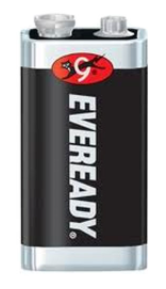
\includegraphics[width=0.2\textwidth]{Secciones/Desarrollo/pila.png}
    \caption{Batería de 9V}
    \label{fig:pila}
\end{figure}

Es necesario utilizar otro elemento para entregar a la celda de carga la tensión necesaria para su funcionamiento.
Se elige utilizar una fuente de alimentación ajustable LM2596 \autoref{fig:fuente} para disminuir la tensión de 9V a 5V y entregar una tensión estable.
\begin{figure}[H]
    \centering
    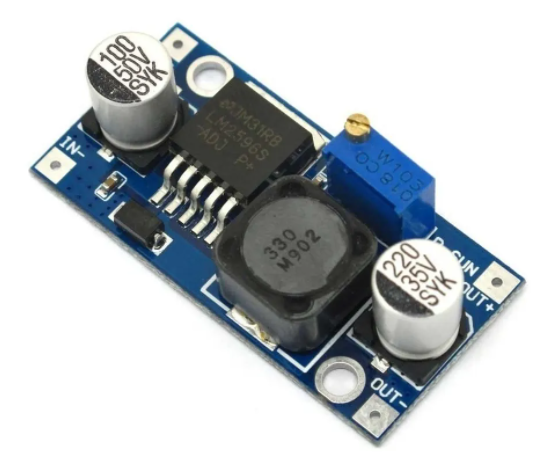
\includegraphics[width=0.5\textwidth]{Secciones/Desarrollo/fuente.png}
    \caption{LM2596}
    \label{fig:fuente}
\end{figure}

\subsubsection{Celda de carga}
La celda de carga elegida es la modelo FH02 \autoref{fig:celda} con la principales características \autoref{fig:celdaData}, es una celda económica y cumple con los
requerimientos de diseño de nuestra balanza comercial.
\begin{figure}[H]
    \centering
    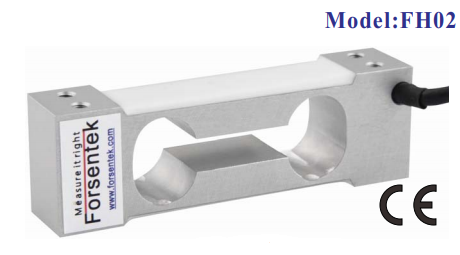
\includegraphics[width=0.5\textwidth]{Secciones/Desarrollo/celda.png}
    \caption{celda de carga:  FH02}
    \label{fig:celda}
\end{figure}
\begin{figure}[H]
    \centering
    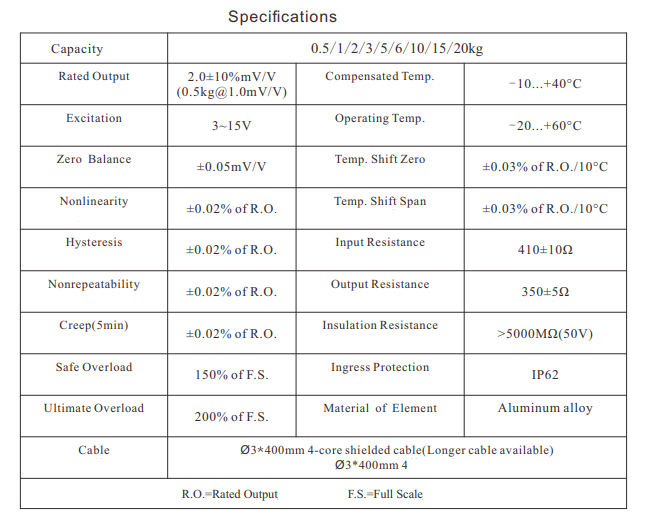
\includegraphics[width=0.8\textwidth]{Secciones/Desarrollo/celdaData.png}
    \caption{}
    \label{fig:celdaData}
\end{figure}
A partir del dato de la tensión de salida nominal se puede calcular la tensión máxima de salida de la celda de carga. Teniendo en cuenta como se dijo anteriormente que se va a alimentar a la celda con 5V se obtiene dado por \autoref{eq:VoCelda}:
\begin{equation*}
    V_{out} = 5~V \cdot 0.2~\frac{mV}{V} = 11~mV
\end{equation*}
Que serán amplificados a un valor de 5 V previo a la lectura del ADC.
\subsubsection{Amplificador de instrumentación}
En la \autoref{fig:amplificadorInstru} se tiene el circuito amplificador que cuenta con 3 amplificadores operacionales, además tiene características tales como una alta impedancia de entrada y una impedancia de fuente que no afecta el cálculo de la ganancia. Como amplificador operacional se elige el modelo AD 8538.
En la \autoref{fig:amplificadorData} se pueden ver el AO y las especificaciones eléctricas principales
del mismo:
\begin{figure}[H]
    \centering
    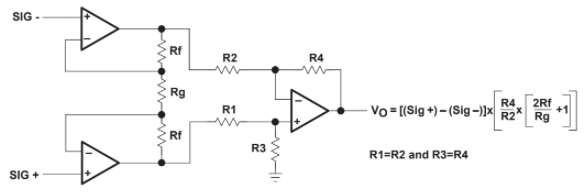
\includegraphics[width=0.9\textwidth]{Secciones/Desarrollo/amplificadorInstru.png}
    \caption{Circuito Amplificador}
    \label{fig:amplificadorInstru}
\end{figure}
\begin{figure}[H]
    \centering
    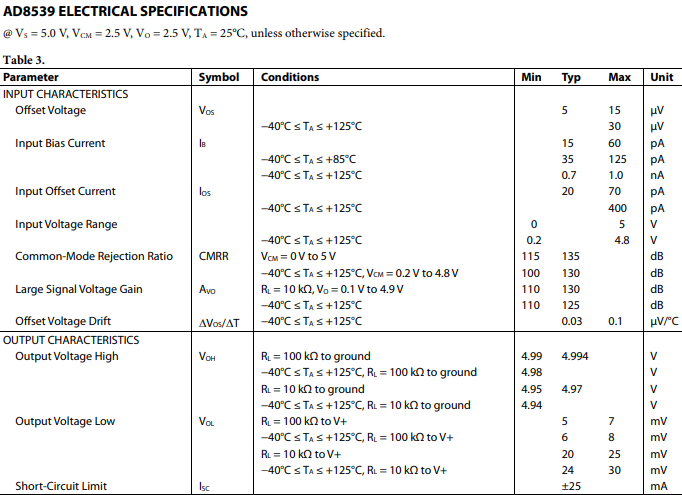
\includegraphics[width=0.9\textwidth]{Secciones/Desarrollo/amplificadorData.png}
    \caption{AD 8538}
    \label{fig:amplificadorData}
\end{figure}
Como se mencionó anteriormente se requiere una salida de 5V a partir de una salida de la
celda de carga de 11 mV, entonces, se calcula la ganancia necesaria:
\begin{equation*}
    k = \frac{5 ~V}{11 ~mV} = 454.5
\end{equation*}

Para la obtención de los demás valores del circuito se decide fijar:
\begin{equation*}
    R1 = R2 = R3 = R4 = 2.2~k\Omega \Rightarrow R_f = 220~k\Omega
\end{equation*}
Mientras que para la obtención del valor de $R_g$ se prueba con distintos valores de la misma hasta encontrar la ganancia más cercana a la que se requiere(\autoref{fig:varRG}), encontrando un valor apto de:
\begin{equation*}
    R_g = 1 ~k\Omega
\end{equation*}
\begin{figure}[H]
    \centering
    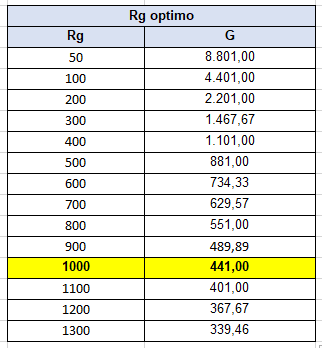
\includegraphics[width=0.7\textwidth]{Secciones/Desarrollo/varRG.png}
    \caption{Variación de Rg}
    \label{fig:varRG}
\end{figure}

\subsection{Errores DC}
Del fabricante obtenemos:
\begin{equation*}
    \begin{aligned}
        &V_{os} = 13~uV\\
        &I_{os} = 50~pA\\
        &I_{pol+} = 50~pV\\
        &I_{pol-} = 0~pV\\
        &RRMC = 31.26 M\\
        &A_d = 11.22M\\
        &R = 125~\Omega\\
        &F_s = 5~V\\
        &V_{cm} = 2.5~V\\
    \end{aligned}
\end{equation*}
\subsubsection{Errores para el amplificador N°1}
\begin{equation*}
    \begin{aligned}
        &T_1=\left(-A_d\right) *\left(\frac{R_f+R_g}{2 R_f+R_g}\right)=(-11.22 M) * \frac{(220 k \Omega+1000 \Omega)}{(2 * 220 k \Omega+1000 \Omega)}=-5.62 ~M \\
        &A_{O L 1}=A_d=11.22 M \\
        &A_{C L 1}=\frac{A_{o L 1}}{1-T_1}=\frac{11.22 ~M}{1+5.62~ M}=2 \\
        &A_{C L 3}=-\frac{R_4}{R_2}=-\frac{2.2 k \Omega}{2.2~ k \Omega}=-1
    \end{aligned}
\end{equation*}
\paragraph{Error por tensión de offset}
    \begin{equation*}
        \Delta V_{o s}=V_{o s} * A_{C L 1} * A_{C L 3}=13 u V * 2 *(-1)=-25.94 ~\mu V
    \end{equation*}
\paragraph{Error por corriente de polarización}
    \begin{equation*}
        \Delta V_{I_{p o l}}=I_{p o l+} * \frac{R}{2} * A_{C L 1} * A_{C L 3}=50~ p A * \frac{125 \Omega}{2} * 2 *(-1)=-6.24 ~n V
    \end{equation*}
\paragraph{Error por ganancia de lazo abierto finita}
    \begin{equation*}
        \Delta V_{A_d}=\frac{F_s}{1-T_1} * A_{C L 3}=\frac{5 \mathrm{~V}}{1+5.62 \mathrm{M}} *-1=889.23~ \mathrm{nV}
    \end{equation*}
\paragraph{Error por RRMC finita}
    \begin{equation*}
        \Delta V_{R R M C}=\frac{V_{c m} * A_{c L 1}}{R R M C}=\frac{2.5 ~V * 2}{31.62 M}=157.76 ~\mathrm{nV}
    \end{equation*}
\paragraph{Error total}
    \begin{equation*}
        \Delta V_1=\Delta V_{o s}+\Delta V_{I_{p o l}}+\Delta V_{A_d}+\Delta V_{R R M C}=26.99 ~\mu \mathrm{V}
    \end{equation*}
\subsubsection{Errores para el amplificador N°2}
\begin{equation*}
    \begin{aligned}
        &T_2=\left(-A_d\right) *\left(\frac{R_f+R_g}{2 R_f+R_g}\right)=(-11.22 M) * \frac{(220~ k \Omega+1000 \Omega)}{(2 * 220 k \Omega+1000 \Omega)}=-5.62 ~M \\
        &A_{O L 1}=11.22 ~M \\
        &A_{C L 1}=\frac{A_{o L 1}}{1-T_1}=\frac{11.22 M}{1+5.62 M}=2 \\
        &A_{C L 3}=\left(\frac{R_3}{R_1+R_3}\right) *\left(\frac{1+R_4}{R_2}\right)=\left(\frac{2.2 k \Omega}{2.2 k \Omega+2.2 k \Omega}\right) *\left(1+\frac{2.2 k \Omega}{2.2 k \Omega}\right)=1
    \end{aligned}
\end{equation*}
\paragraph{Error por tensión de offset}
    \begin{equation*}
        \Delta V_{o s}=V_{o s} * A_{C L 1} * A_{C L 3}=13 u V * 2 * 1=25.94 ~\mu V
    \end{equation*}
\paragraph{Error por corriente de polarización}
    \begin{equation*}
        \Delta V_{I_{p o l}}=I_{p o l+} * \frac{R}{2} * A_{C L 1} * A_{C L 3}=50 p A * \frac{125 \Omega}{2} * 2 *1=6.24 ~n V
    \end{equation*}
\paragraph{Error por ganancia de lazo abierto finita}
    \begin{equation*}
        \Delta V_{A_d}=\frac{F_s}{1-T_2} * A_{C L 3}=\frac{5 \mathrm{~V}}{1+5.62 \mathrm{M}} * 1=889.23~ \mathrm{nV}
    \end{equation*}
\paragraph{Error por RRMC finita}
    \begin{equation*}
        \Delta V_{R R M C}=\frac{V_{c m} * A_{c L 1}}{R R M C}=\frac{2.5~ V * 2}{31.62 M}=157.76 ~\mathrm{nV}
    \end{equation*}    
\paragraph{Error total}
    \begin{equation*}
            \Delta V_2=\Delta V_{o s}+\Delta V_{I_{\text {pol }}}+\Delta V_{A_d}+\Delta V_{R R M C} = 26.99 ~u V
    \end{equation*}
\subsubsection{Errores para el amplificador N°3}
\begin{equation*}
        T_3=\left(-A_d\right) *\left(\frac{R_2}{R_2+R_4}\right)=(-11.22 M) * \frac{2.2~ k \Omega}{(2.2~ k \Omega+2.2~ k \Omega)}=-5.61 ~M \\
\end{equation*}
\paragraph{Error por tensión de offset}
\begin{equation*}
    \Delta V_{o s}=V_{o s} *\left(1+\frac{R_4}{R_2}\right)=13 ~u V *\left(1+\frac{2.2 ~k \Omega}{2.2 ~k \Omega}\right)=26 ~u V
\end{equation*}
\paragraph{Error por corriente de polarización}
\begin{equation*}
    \Delta V_{I_{p o l}}=\left(\frac{R_1 * R_3}{R_1+R_3}\right) * A_d * \frac{I_{o s}}{1-T_3} \approx R_3 * I_{o s}=2.2 ~k \Omega * 50 ~p A=110 ~\mathrm{nV}
\end{equation*}
\paragraph{Error por ganancia de lazo abierto finita}
\begin{equation*}
    \Delta V_{A_d}=\frac{F_s}{1-T_3}=\frac{5 ~\mathrm{V}}{1+5.62 \mathrm{M}} =891.25~ \mathrm{nV}
\end{equation*}
\paragraph{Error por RRMC finita}
    \begin{equation*}
        \Delta V_{R R M C}=\frac{F_s}{RRMC}= \frac{5~V}{31.26M} = 157.11 ~\mathrm{nV}
    \end{equation*}
\paragraph{Error total}
\begin{equation*}
    \Delta V_3=\Delta V_{o s}+\Delta V_{I_{\text {pol }}}+\Delta V_{A_d}+\Delta V_{R R M C} = 27.16 ~u V
\end{equation*}  
\subsubsection{Tabla resumen de Errores}
\begin{table}[H]
\centering
\caption{Resumen de errores.}
\label{tab:my-table}
\begin{tabular}{|c|c|c|c|}
\hline
\multicolumn{1}{|l|}{} & \cellcolor[HTML]{FFCC67}Amplificadores & \multicolumn{1}{l|}{\cellcolor[HTML]{FFCC67}} & \multicolumn{1}{l|}{\cellcolor[HTML]{FFCC67}} \\ \hline
\rowcolor[HTML]{FFCC67} 
\cellcolor[HTML]{F8FF00}Errores & Nº1 & Nº2 & Nº3 \\ \hline
\cellcolor[HTML]{F8FF00}$\Delta V_{o s}$ & -25.94 uV & 25.94 uV & 26 uV \\ \hline
\cellcolor[HTML]{F8FF00}$\Delta V_{I_{p o l}}$ & -6.24 nV & 6.24 nV & 110 nV \\ \hline
\cellcolor[HTML]{F8FF00}$\Delta V_{A_d}$ & -889.23 nV & 889.25 nV & 891.25 nV \\ \hline
\cellcolor[HTML]{F8FF00}$\Delta V_{R R M C}$ & 151.76 nV & 157.76 nV & 157.11 nV \\ \hline
\rowcolor[HTML]{34FF34} 
\cellcolor[HTML]{F8FF00}$\Delta V_x$ & \textbf{26.99 uV} & \textbf{26.99 uV} & \textbf{27,16 uV} \\ \hline
\end{tabular}
\end{table}

Tenemos un valor de error total de:
\begin{equation*}
    \Delta V = \Delta V_1 + \Delta V_2 + \Delta V_3 = 81.15 ~uV
\end{equation*}
\subsection{Errores debido a la temperatura}
\subsubsection{Drift de Ganancia}
La Ganancia del amplificador de instrumentación es:
\begin{equation*}
    A_{AI} = \left(\frac{R2}{R4}\right) \left(\frac{2Rf}{Rg} + 1\right)
\end{equation*}
Para evitar que esta ganancia varíe con los cambios de la temperatura se deben usar
resistencias con el mismo coeficiente de temperatura. En este caso se escogieron resistencias
MFS1/4D con un coeficiente de temperatura de 100 ppm/ºC sí casi no se introducen errores extras, al menos en este aspecto.
\subsubsection{Drift de Vos}
El voltaje de offset varía con la temperatura, según la hoja de datos del amplificador este
tiene un valor de:
\begin{equation*}
    \frac{\Delta V_{os}}{\Delta T} = 0.1 \frac{uV}{ºC}
\end{equation*}

Multiplicando por $T_{max} = 40ºC$ para la aplicación resulta:
\begin{equation*}
\Delta V_{o s}=0.1 \frac{\mu V}{{ }^{\circ} \mathrm{C}} * 40^{\circ} \mathrm{C}=4 \mu V \rightarrow \frac{\Delta V_{o s}}{V_{o s}}=0.31
\end{equation*}
Entonces por proporción los errores a la salida en DC debido a Vos, que se calcularon antes,
se incrementan un 31\% debido a la temperatura. Dicha variación se calcula para cada AO:

\begin{equation*}
    \begin{aligned}
    &\Delta V_{o s 1}=0.31 \Delta V_{o s 1(D C)}=0.31 * 25.94 \mu V=7.98 \mu V \\
    &\Delta V_{o s 2}=7.98 \mu V \\
    &\Delta V_{o s 3}=8 \mu V \\
    &\Delta V_{t o t}=23.96 \mu V
    \end{aligned}
\end{equation*}
\subsection{Número de bits del conversor}
Con el valor del fondo de escala y el error total se puede calcular la resolución necesaria del
conversor y se expresa de la siguiente manera: 
\begin{equation*}
    \begin{aligned}
    &\Delta V_{T O T}=\Delta V_{D C}+\Delta V_{T e m p}=81.15 \mu V+23.96 \mu V=105.11 \mu V \\
    &n=\log _2\left(\frac{F_S}{\Delta V_{T O T}}\right)=15.53 \text { bits } \rightarrow 15 \text { bits }
    \end{aligned}
\end{equation*}
Como se tiene un conversor con un número de bits mayor a 11 bits (2048) entonces este es
compatible con la resolución de 1 gramo provista en las especificaciones técnicas de la
balanza a diseñar.
\subsubsection{Simulaciones}

\begin{figure}[H]
    \centering
    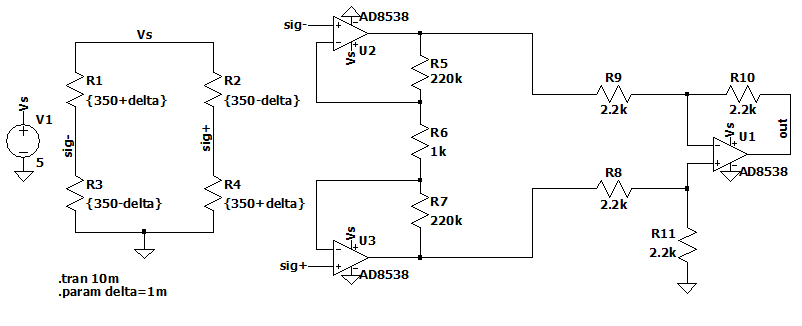
\includegraphics[width=0.9\textwidth]{Secciones/Desarrollo/circ1.png}
    \caption{Circuito de simulación}
    \label{fig:circ1}
\end{figure}
\subsubsection{Simulaciones punto de DC para un puente balanceado}
\begin{figure}[H]
    \centering
    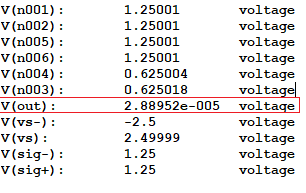
\includegraphics[width=0.8\textwidth]{Secciones/Desarrollo/simuDC.png}
    \caption{DC point}
    \label{fig:simuDC}
\end{figure}
Al no tener entrada diferencial, la salida distinta de cero corresponde a los errores de DC,
recordando que los errores producidos por el AO1 y AO2, son en realidad de igual magnitud y
de signo opuesto, por lo que solo quedan los errores producidos por AO3. Donde lo calculado
es muy similar a los visto en los resultados de la simulación.
\subsubsection{Simulaciones punto de DC para un puente desbalanceado}
\begin{figure}[H]
    \centering
    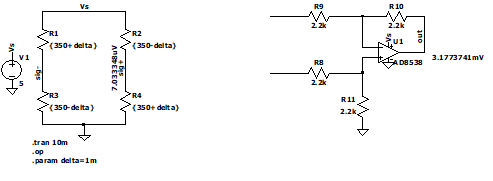
\includegraphics[width=0.9\textwidth]{Secciones/Desarrollo/circ2.png}
    \caption{}
    \label{fig:circ2}
\end{figure}
En la imagen de la izquierda se ve el puente con un desbalance debido a una deformación que
produjo un cambio de $1~m\Omega$ en las resistencias del puente, se observa una tensión diferencial. A la derecha se muestra la salida del amplificador de instrumentación.

\begin{equation*}
    \begin{aligned}
    &V_{\text {dif }}=\operatorname{sig}_{+}-\operatorname{sig}{ }_{-}=7.033348 \mu \mathrm{V}\\
    &V_{\text {out }}=3.1773741 \mathrm{mV}\\
    &A_{A I}=\frac{V_{\text {out }}}{V_{d i f}}=451.7
    \end{aligned}
\end{equation*}
\subsection{Calculo económico}
Los valores obtenidos se tomaron en dolares.
\begin{figure}[H]
    \centering
    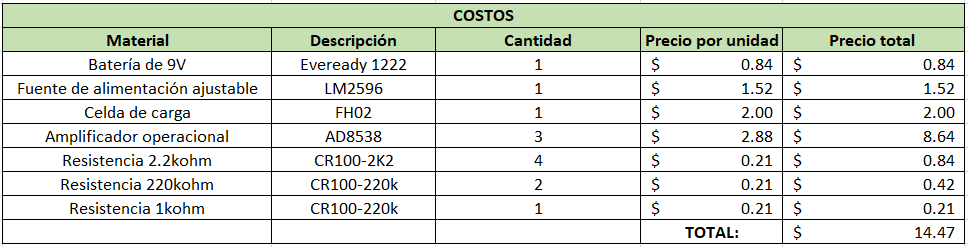
\includegraphics[width=0.9\textwidth]{Secciones/Desarrollo/costos.png}
    \caption{}
    \label{fig:costos}
\end{figure}
Como se puede observar el valor total del material utilizado ronda los 14.5 dólares, este valor
multiplicado al precio del dólar blue de hoy (290) se transforma en 4060 pesos.
